\chapter{The \Fermi{ }Gamma-Ray Space Telescope and \gam{} Data Analysis}
\label{chap:FGST}

\section{\label{FGST:intro}Introduction}
The \Fermi{} Gamma-Ray Space Telescope (\Fermi{} ~hereafter), successor to the \egret{} instrument on the \cgro{}, was successfully launched into orbit around Earth on June 11 2008. \Fermi{} consists of two instruments, the \lat{} and the \gbm{}. The \lat{}, which is the primary instrument on \Fermi{}, is a pair conversion telescope designed to detect photons from 20\mev{} to greater than 1\tev{} \cite{atwood09, lat_perf, 2FHL} Its standard mode of operation is a sky-survey mode in which it observes the entire sky every 3 hours. The secondary instrument aboard \Fermi{}, the \gbm{}, was designed to detect \gam{} bursts in a waveband overlapping that of the \lat{} yet complementary in that its energy extends considerably lower. Combined the \lat{} and \gbm{} comprise a formidable observatory, spanning more than 8 decades in energy, and it is currently the only instrument performing all-sky observation in this broad energy range. 

\begin{figure*}[!]
	\begin{center}
		\hspace*{-1.5cm} \begin{tabular}{ll}
			\includegraphics[width=6.5cm]{Figures/{231388main_fairopen-lg_full}.jpg} &
			\includegraphics[width=6.5cm]{Figures/{glast_readytogo}.jpg} \\
			
			\includegraphics[width=6.5cm]{Figures/{seth_02}.jpg} &
			\includegraphics[width=6.5cm]{Figures/{seth_2356}.jpg} \\

		\end{tabular}
	\end{center}
	\caption[\Fermi{} launch images.]{
		\label{fig:Launch}{Top left: \Fermi{} being loaded on to a Delta II 7920-H rocket after arriving at Cape Canaveral. Top right: Delta II rocket  at Space Launch Complex 17B with \Fermi{} on board. Lower Left: Dr. Elizabeth Hays at Cape Canaveral marveling at the majestic launch of the \Fermi{} observatory. Lower right:.\Fermi{} was launched into a 550 km, low Earth orbit, on June 11 2008, at 16:05 UTC. Images courtesy of NASA and Seth Diegel.}
	}
\end{figure*}

\section{\label{FGST:LAT}The Large Area Telescope}
Due the the nature of interaction between \gam{}s and matter, photons of \gam{} energies cannot be reflected or refracted in the same way as lower energy light can be, which restricts the design possibilities of a \gam{} telescope. Because of this limitation, \Fermi{} uses the photon pair-production phenomenon to detect \gam{} photons. Photon pair production refers to the mechanism by which a
photon with sufficient energy (at least twice the rest mass of an electron) can convert to an electron/positron pair. The conversion from photon to antimatter pair can only occur in the presence of a nucleus whose Coulomb field can absorb and thus conserve the momentum of the photon. Figure \ref{fig:pairProd} top shows the probability of photon conversion for given energies, demonstrating how higher Z (and thus stronger field) nuclei, are more conducive to conversion by providing a larger interaction cross section. Figure \ref{fig:pairProd} bottom plots the interaction cross section versus photon energy. Above 10 \mev{}, photon pair production (${\rm \kappa_{nuc}}$) is the clearly dominant photon interaction process \cite{Beringer12}.

\begin{figure}[!]
	\centering
	\vspace{-0.5cm}
		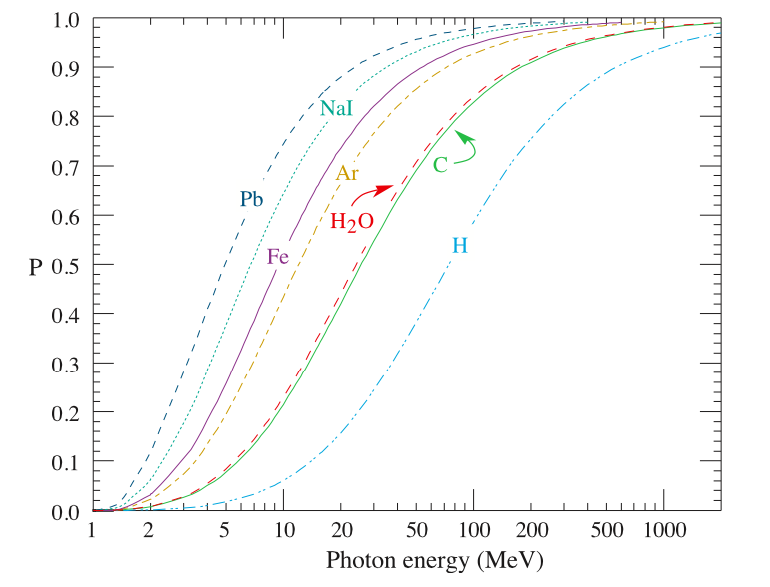
\includegraphics[width=0.85\columnwidth]{Figures/Beringer12_30_17.png}
		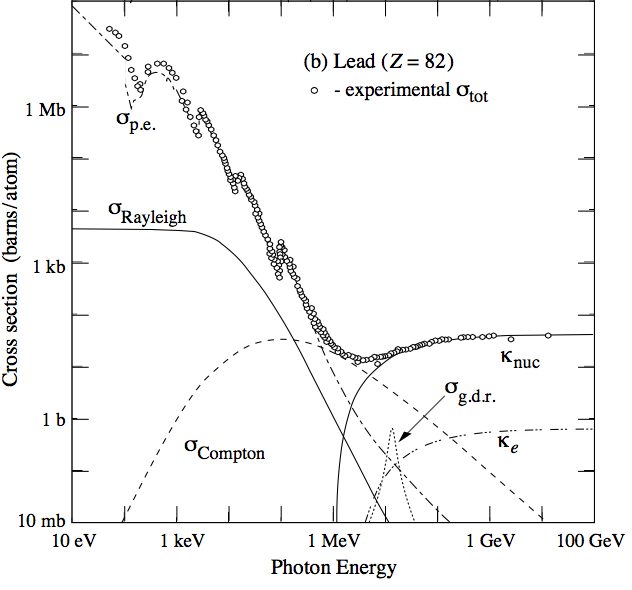
\includegraphics[width=0.85\columnwidth]{Figures/Beringer12_30_15.png}
	\caption[Top:Probability of photon conversion to e$^-$ e$^+$ pair. Bottom: Photon cross section versus energy]{Top: Probability that a photon interacting with various nuclei will result in an \ee{} pair as a function of energy. Bottom: Photon cross section versus energy for various photon-matter interaction channels. Both figures originally from \cite{Beringer12} as Figure 30.17 and 30.15.}
	\label{fig:pairProd}
\end{figure}

The \lat{} instrument on board \Fermi{} is composed of three subsystems, all designed to take advantage of the pair production mechanism. First and foremost, is the \tkr{}. The \lat{}'s \tkr{} is a module consisting of 18 x-y paired silicon strip detectors that measure the trajectories of the pair-produced charged particles. The silicon strips are interleaved with a tungsten foil to promote \gam{}s passing through the material to convert to \ee{} pairs. The \lat{} is made up of 16 towers (arranged in a 4x4 grid), with each tower containing the 18 interlaced silicon, tungsten planes. The top 12 layers of the \tkr{} comprise the "front section" and are made of 3\% radiation length tungsten. The next 4 layers constitute the "back section" of the \tkr{} and are made of thicker, 18\% radiation length tungsten foil. The final two \tkr{} layers contain no tungsten and are present as a requirement of the \tkr{} trigger which requires at least three hits in adjacent layers to trigger \cite{lat_perf}. The front section of the \tkr{} was designed to minimize the separation between tungsten and silicon (\ie{}\ the point of conversion and subsequent detection) minimizing multiple scattering effects therein, and thus optimizing the \psf{} for events converted in this section. The 6-times-thicker back layers were designed to further promote conversion, maximizing the effective area of the \lat{}, yet sacrificing resolution for events converting in this layer. Figure \ref{fig:Tower}, shows a diagram of a single tower with \tkr{} components included.


The next subsystem of the \lat{} is the \calo{}. The \calo{} (located at the bottom of each of the 16 towers as in Figure \ref{fig:Tower}) is comprised of 96 CsI scintillation crystals, arranged in 8 layers of 12 logs. This construction allows the \calo{} to {\bf 1.} measure the energy deposition of the shower of particles resulting from the incident photon's pair-produced \ee{} pair, and {\bf 2.} to perform 3D imaging of the shower, which can serve as a measurement of shower energy leakage.

\begin{figure}[h!t]
	\centering
	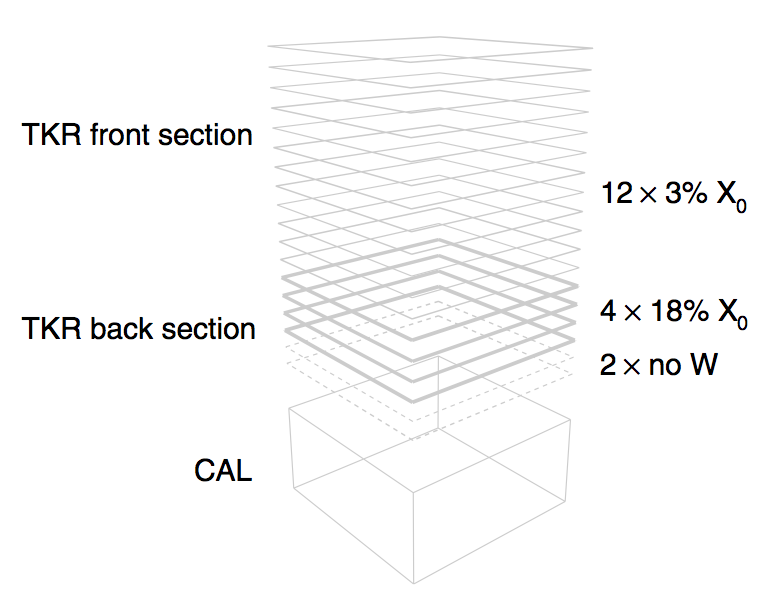
\includegraphics[width=1.0\columnwidth]{Figures/latPerf_Tower.png}
	\caption[LAT tower schematic ]{\lat{} tower schematic showing the different \tkr{}layers and ending with the \calo{} on the bottom of the tower. Taken from \cite{lat_perf}}
	\label{fig:Tower}
\end{figure}

The final vital component of the \lat{} is the \acd{}. The role of the \acd{} is to reject background charged particles that enter the \lat{} to avoid misclassifying them as photons. The design of the \acd{} was informed by lessons learned from the \lat{}'s predecessor, the \egret{} instrument on \cgro{} \citep{Mosieev05}. In the \calo{} the electromagnetic shower generated by the incident photon produces secondary particles as well as X-rays. These X-rays can Compton scatter the charged particles out through the 
\tkr{} and \acd{} (referred to as ``backsplash'') creating false vetoes. This backsplash was present in \egret{} and reduced the efficiency of the instrument above 10 GeV \cite{atwood09}. To overcome the backsplash effect, the \lat{} uses a segmented rather than monolithic layer for the \acd{}, made up of 89 scintillating tiles surrounding the towers (as in Figure \ref{fig:latGuts}).

\begin{figure}[ht!]
	\centering
	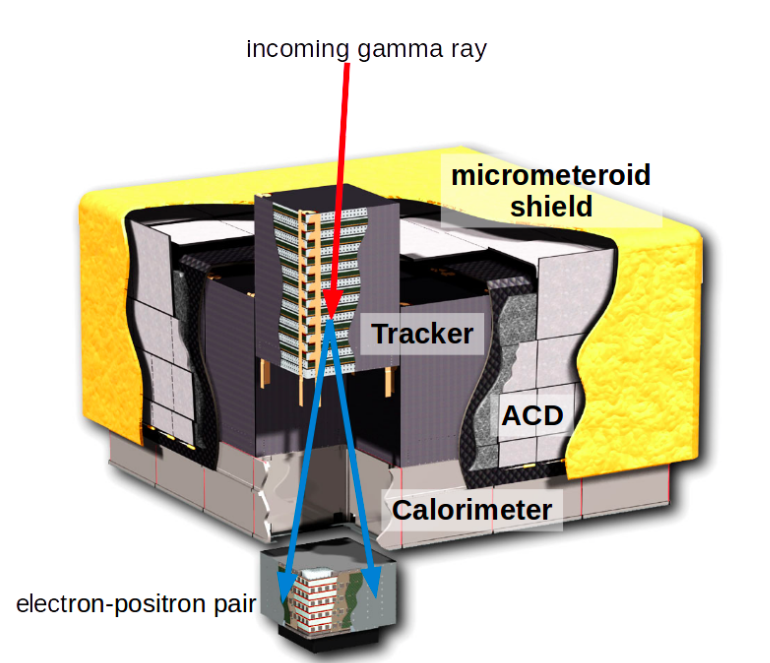
\includegraphics[width=1.0\columnwidth]{Figures/latGuts.png}
	\caption[Diagram of the three primary LAT subsytems.]{Diagram of the \lat{} subsystems demonstrating how an incident \gam{} can enter through the top layer of the \acd{}, convert to a \ee{} pair in a layer of the \tkr{}, and finally deposit its energy in the \calo{}.}
	\label{fig:latGuts}
\end{figure}
 
\section{\label{FGST:analysis}LAT Performance}
The \lat{} performance is dictated by the telescopes hardware and software designs (\eg{}\  event reconstruction methods, background and event classifications). The parameterizations of the performance are referred to as the \irf{}. The \lat{} \irf{} are factorized into three terms:
\begin{enumerate}
	\item {\bfseries \psf{}, P${\mathbf{(\hat{v^\prime};E,\hat{v})}}$:} Represents the angular resolution of the \lat{}. It is the probability density for reconstructing an incident \gam{} with position $\hat{v^\prime}$ if the true position is $\hat{v}$ for given energy E. The \psf{} is strongly energy dependent. At low energies, this dependence is dominated by multiple scattering in the \tkr{} causing the \psf{} to broaden, and at higher energies (above a few \gev{}) it is dominated by the strip pitch, or the distance between adjacent silicon strip centers, which limits how fine the \psf{} can be at high energies.
	
	\begin{figure*}[ht]
		\begin{center}
			\includegraphics[width=1.\columnwidth]{Figures/{gPsfAve95Energy_P8R2_SOURCE_V6fb_10MeV}.png}
		\end{center}
		\caption[LAT P8R2\_SOURCE\_V6 angular resolution.]{
			\label{fig:PSF}{\lat{} angular resolution for 68\% and 95\% containment radius and front and back converting events as a function of energy for the P8R2\_SOURCE\_V6 event classification. Figure from \url{https://www.slac.stanford.edu/exp/glast/groups/canda/lat_Performance.htm}}}
	\end{figure*}
	
	\item {\bfseries Effective Area, A${\mathbf{ _{eff}(E,\hat{v})}}$}: Represents the collecting area of the \lat{}. It is the product of the geometric cross section of the \lat{} and a dimensionless term that quantifies the efficiency of the \lat{}'s event reconstruction. It has units of area. 
	
	\begin{figure*}[ht]
			\begin{center}
				\includegraphics[width=1.\columnwidth]{Figures/{gAeffEnergy_P8R2_SOURCE_V6fb_10MeV}.png}
			\end{center}
			\caption[LAT P8R2\_SOURCE\_V6 effective area]{
				\label{fig:Aeff}{\lat{} effective area for front, back, and total converting events as a function of energy for the P8R2\_SOURCE\_V6 event classification. Figure from \url{https://www.slac.stanford.edu/exp/glast/groups/canda/lat_Performance.htm}.}}
	\end{figure*}
	
	\item {\bfseries Energy Dispersion, D${\mathbf{(\hat{E^\prime};E,\hat{v})}}$}: Represents the energy resolution of the \lat{}. It is the probability density for reconstructing an incident \gam{} with energy $\hat{E^\prime}$ if the true energy is $\hat{E}$ for given direction on the sky. Energy dispersion effects are often ignored in \lat{} analysis above a few hundred \mev{} as \cite{lat_perf} showed that the effects of neglecting it are of the order of a few percent.
	
		\begin{figure*}[ht]
			\begin{center}
				\includegraphics[width=1.\columnwidth]{Figures/{gEdispAve68Energy_P8R2_SOURCE_V6fb_sep_10MeV}.png}
			\end{center}
			\caption[LAT P8R2\_SOURCE\_V6 energy resolution]{
				\label{fig:Edisp}{\lat{} energy resolution for front, back, and total converting events as a function of energy for the P8R2\_SOURCE\_V6 event classification. Figure from \url{https://www.slac.stanford.edu/exp/glast/groups/canda/lat_Performance.htm}.}}
		\end{figure*}
	
\end{enumerate}

In general, the \lat{} has a large effective area (${\rm \sim 9500 cm^2}$ at a few \gev{}) (Figure \ref{fig:Aeff}), energy resolution of 5\% (at 10 \gev{}) to 20\% (at 100 \mev{}) (Figure \ref{fig:Edisp}), and a single-photon angular resolution ranging from $\sim 3.2^\circ$ at 100 \mev{} to $
\lesssim 0.16^\circ$ for E $>$ 10 \gev{} (Figure \ref{fig:PSF}). With its rocking mode observation strategy (35$^\circ$ north of the zenith axis for one orbit, and then south for the next) and its  wide \fov{} of 2.4 sr, the \lat{} attains a nearly uniform coverage of the sky within two orbits, or 3 hours. The culmination of the \lat{}'s performance can be summed up as its capability to detect distinct sources on the sky. Figures \ref{fig:sensMap} and \ref{fig:sensSlice} depict the \lat{}'s threshold for detecting emission from a point source above the structured Galactic diffuse emission \ref{gamAstr:Sources}. Figure \ref{fig:sensMap} demonstrates what level of emission the \lat{} can detect when integrating over the majority of its energy range, and Figure \ref{fig:sensSlice} shows what the  source detection threshold is for detecting sources in individual energy bins and at four locations on the sky. See \ref{Rems:latGam} for a comparison of the \lat{}'s capabilities with that of \egret{}.

\begin{figure*}[!ht]
	%\begin{centering}
	\hspace{-2.7cm}
	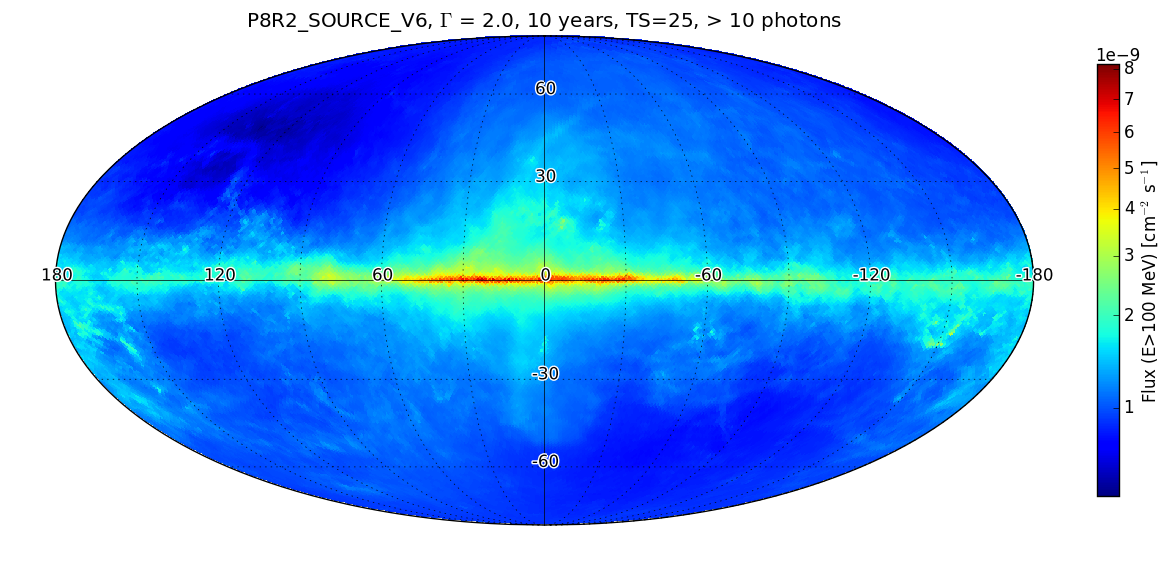
\includegraphics[width=1.3\columnwidth]{Figures/allsky_flux_sensitivity_p8r2_source_v6_all_10yr_zmax100_powerlaw_g200_n10_ts25.png}
	\caption[LAT 10 year, P8R2\_SOURCE\_V6 integral-flux sensitivity map]{\lat{} 10 year, integral-flux sensitivity map for P8R2\_SOURCE\_V6 event classification. The all-sky map was created for energies above 100\mev{} and for a point source (modeled as a \pl{} of spectral index 2) to obtain a $5\sigma$ significance. Figure from \url{https://www.slac.stanford.edu/exp/glast/groups/canda/lat_Performance.htm}.
		\label{fig:sensMap}}
	%\end{centering}
\end{figure*}

\begin{figure*}[!ht]
	\begin{centering}
		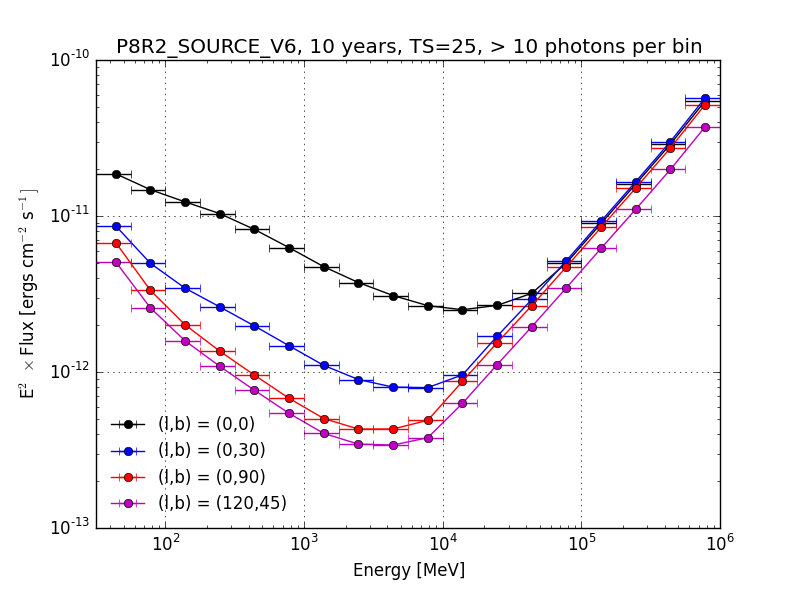
\includegraphics[width=1.0\columnwidth]{{Figures/differential_flux_sensitivity_p8r2_source_v6_all_10yr_zmax100_n10.0_e1.50_ts25}.png}
		\caption[LAT 10 year, P8R2\_SOURCE\_V6 differential-flux sensitivity for four locations on the sky.]{\lat{} 10 year, differential-flux sensitivity map for P8R2\_SOURCE\_V6 event classification. The all-sky map was created for energies above 100 \mev{} and for a point source (modeled as a \pl{} of spectral index 2) to obtain a $5\sigma$ significance. Figure from \url{https://www.slac.stanford.edu/exp/glast/groups/canda/lat_Performance.htm}.
			\label{fig:sensSlice}}
	\end{centering}
\end{figure*}

For a given \gam{} source model $S(E,\hat{p})$, \ie{}\ the number of photons per unit time, energy, and solid angle at a given time, energy, and position on the sky, where $\hat{p}$ is the direction on the sky, we can convolve the source model (times the effective area) with the dispersion components (\psf{} and  energy dispersion) to obtain the predicted differential source counts (in counts per unit energy/time/solid angle) by integrating over the energy and time range of interest and over the solid angle in the \lat{} reference frame:
\begin{align}\label{eq:exCountsPred}
	M(E^{\,\prime},\hat{p}^{\,\prime}) =  \int \int \int S(E,\hat{p}) A _{eff}(E,\hat{v}) \times \nonumber \\
	P(\hat{v}'(t,\hat{p}^{\,\prime}); E, \hat{v}(t;\hat{p})) D(E^{\,\prime}; E, \hat{v}(t;\hat{p})) dE d\Omega dt.
\end{align}

All the values discussed above are particular to the recent \lat{} event-level reconstruction update colloquially referred to as Pass 8 \citep{atwood13}. Pass 8 consists of a series of improvements to the \lat{}'s event selection process. The three primary areas of improvement are in the event reconstruction methods, background rejection, and Monte carlo simulations of the detector using flight data. One improvement example involves the way in which the that \lat{} reconstructs and tracks the path of an \ee{} pair back to an incident photon. Previously a track-by-track pattern recognition algorithm was used to find the two antimatter paths and combine them back to determine the vertex of conversion. The improved method uses a tree-based tracking method that considers conversion in the \tkr{} as the start of an electromagnetic shower and attempts to model this process by grouping hits in the \tkr{} into one or more ``trees". Similar event reconstruction methods have also been applied to the \acd{} and \calo{}. 

The combined effects of the various upgrades result in an extension of the energy down to 30\mev{} and up to 3\tev{} \cite[see Chapter \ref{chap:2FHL} for applications]{Bruel12}, a 40\% gain in point-source sensitivity, up to a 2$\times$ increase in acceptance (defined as effective area integrated over solid angle) below 100\mev{} and above 100\gev{}, and a narrower \psf{} at high energies. Several new event classifications have also been developed (in addition to the previous front and back event types) to leverage the newfound  Pass 8 \lat{} capabilities. Specifically, there are new event types that define the quality of event reconstruction for both the \psf{} and energy dispersion, by partitioning events into quartiles based on quality, allowing for an even finer grade energy and spatial resolution.

%\begin{equation}\label{eq:exposureDef}
%\mathcal{E}(E,\hat{p},s) = \int  A _{eff}(E,\hat{v}) dt.
%\end{equation}

%\begin{equation}\label{eq:tobsDef}
%\mathcal{E}(E,\hat{p},s) = \int  A _{eff}(E,\hat{v}) t_{obs}(\hat{v};\hat{p}) d\Omega.
%\end{equation}


\section{\label{FGST:analysis}\FermiLat{} Data Analysis Method}
The standard method for analyzing astrophysical data at other wavelengths (\eg{}\ optical) is by performing aperture photometry. This consists of essentially counting the photons ``on-source'' in a extraction region and subtracting off the estimated background ``off-source'' in a neighboring region, where the background is typically assumed to be isotropic. Although not always simple, various source quantities can typically be derived from the data itself (\eg{}\ intensity, extent if resolvable). The aperture photometry method is not feasible for analysis of \Fermi{} data (as was the case for \egret{} \cite{mattox96}) due to various complexities inherent to detecting \gam{} photons. 

The first such issue is that because of the breadth of the \lat{} \psf{}, and wide energy range of the \lat{}. Due to these factors, source confusion abounds and sources are not truly isolated from one another. The overlapping tails of the \psf{} would make analysis via aperture photometry particularly intractable at low energies (where the \psf{} rises steeply with decreasing energy, see Figure \ref{fig:PSF}) and in the Galactic plane (with a high source density and strongly anisotropic diffuse emission \ref{FGST:diff?}).The second reason is the complex relationship between an individual source and the \irf{}. Since \Fermi{} typically operates in a sky-survey mode, photons from an individual source need to accumulate over long integration times, and the orientation of the space craft with respect to the source of interest will vacillate over time. The response of the telescope is dependent on the orientation of the space craft, so it is non-trivial to determine source and background fluxes by simply counting photons.

To circumvent the issues described above, \cite{Cash79} applied the maximum likelihood method to astrophysical counting-experiments and parameter estimation of X-ray data. \cite{mattox96} then established a framework for analyzing \egret{} \gam{} via the maximum likelihood method. The likelihood, \like{}, is defined as the probability of obtaining the data observed assuming a model of the sky. In the maximum likelihood framework, we want to estimate the model parameters by maximizing the likelihood and finding the  parameters that best-fit the data. Since the \lat{} is a particle detector, and hence a photon counting experiment, the observed counts are distributed as a Poisson distribution with unknown mean. For large data sets it is more tractable to use a binned maximum likelihood analysis; binning in both position on the sky and energy. The binned maximum likelihood function for \lat{} is thus given as:
\begin{equation}\label{eq:posLike}
{\rm \like{} = \prod_{i} \frac{m_i^{n_j}e^{-m^i}}{n_i!}}
\end{equation}
Thus the likelihood is the product of the Poisson probabilities over all j positions and energies, where ${\rm m_i}$ is the expected counts in the i\textsuperscript{th} bin, and ${\rm n_i}$ is the observed counts in the i\textsuperscript{th} bin.  It is often computationally easier to work with the log of the likelihood, so taking the log of \ref{eq:posLike} gives:

\begin{equation}\label{eq:like}
{\rm \logL{} = -\sum_{i} m_i + \sum_{i} n_j~log~m_j}
\end{equation}
Dropping the arbitrary constant  ${\rm -log~n_i!}$. The term $\sum_{i} m_j $ is the total expected counts in all bins. The model counts ${\rm m_i}$ are calculated by integrating the differential source model (given by \ref{eq:exCountsPred}) over the i\textsuperscript{th} bin for all sources. The \Fermi{} Science Tools were designed to perform the tasks involved in binning the sky in position and energy, calculating the convolution integral in \ref{eq:exCountsPred}, and computing the likelihood of \ref{eq:like} (implemented via {\tt gtbin, gtsrcmaps, and gtlike} respectively).

The other way in which \Fermi{} employs the maximum likelihood method is through the \lrt{} to asses detection source significance and compare model hypotheses. The \lrt{} is a statistical method to assess the goodness-of-fit of two different models. The likelihood is calculated for two models, one of which can be reduced to the other hypothesis under certain conditions. If the more complex model can be reduced to the simpler model (called the null hypothesis), we say the simpler hypothesis is nested within the more complex. In the \lrt{}, the \ts{} is defined as: 

\begin{equation}\label{eq:LRT}
\rm \ts{} \equiv 2\log(\like{}(H_1)~/ \like{}(H_0)),
\end{equation}
with ${\rm H_1}$ being the more complex hypothesis and ${\rm H_0}$ the null. \cite{mattox96} detail how by Wilk's theorem, the \ts{} for detection of a point source (with the null hypothesis being that with no source present, or 0 flux) should be distributed as a chi-squared  distribution in the null hypothesis for an increasing sample size, which for photon counting experiments, is the number of events relevant to the parameter being estimated. Specifically, 

\begin{equation}\label{eq:tsPdf}
\rm PDF(\ts{}) = 1/2~\chi^2_1,
\end{equation} 
where PDF(TS) is the probability distribution function for obtaining a specific value of \ts{} and $\chi^2_1$ is the chi-squared  distribution for one degrees of freedom. The factor of 1/2 arises from the fact that the flux of a source is not permitted to be zero, and since negative and positive fluctuations in a parameter's value contribute equally to the \ts{}, half of the distribution is lost with the positive flux restriction. The significance of detection is oft quoted as ${\rm \sigma \approx \sqrt{TS}}$, which is strictly valid only for $\chi^2_1$. More generally, when comparing the likelihood of two models with n degrees of freedom between them, equation \ref{eq:tsPdf} applies, but using  $\chi^2_n$ for n degrees of freedom versus one.

%The model of the sky will contain terms describing the sources (\ie{} the flux density of all the sources in the region, or $S(E,\hat{p})$ in \ref{FGST:LAT}), the background`

